\documentclass{article}

    \usepackage{graphicx}
    \usepackage{booktabs}
    \usepackage{indentfirst}
    \usepackage{float}
    \usepackage{geometry}
        \geometry{
        a4paper,
        total={170mm,257mm},
        left=20mm,
        top=20mm,
        } 
    \usepackage{hyperref}
    % \hypersetup{
    %         colorlinks=true,
    %         linkcolor=blue,
    %         filecolor=magenta,      
    %         urlcolor=cyan,
    % }
    \newcommand {\weblink}[1]{\href{#1}{\textbf{#1}}}
    \renewcommand{\labelitemi}{$\diamond$}
    \title{CS6960 Project Proposal \protect\\ Learning a Code for Approximate Coded Computation Using Neural Networks}
    \author{Zheng Wang}

\begin{document}
        \maketitle

        \section{Basic Information}
        \begin{itemize} 
           \item Project Title: \textbf{\textit{Learning a Code for Approximate Coded Computation Using Neural Networks}}
           \item Group Members:
           \begin{itemize}
               \item \textbf{Zheng Wang}, u1208847, u1208847@utah.edu
           \end{itemize}
           \item Project Github Link: \weblink{https://github.com/GregDobby/CS6960.git}
        \end{itemize}   

        \section{Background and Motivation}
        Machine learning has been applied in a wide variety of cognitive tasks such as image classification, object recognition, and natural language processing. Moreover, with the development of distributed computing, applications can utilize machine learning algorithms by using cloud services that offer machine learning as a service. Cloud service providers typically use a distributed setup with a large number of interconnected servers(compute nodes). However, due to various factors including unreliable compute nodes and transient slowdowns, servers can face temporary unavailability which is called straggler. And stragglers can adversely affect the response time.
    
    Many strategies have been studied to mitigate the influence of stragglers. One natural approach is to add redundancy which utilizes extra resources to aid in recovery from unavailability. Adding redundancy by simply making copies can lead to significant resource overhead. So the coded computation is developed, which extends the use of erasure codes that can add redundancy with much lesser overhead. 
    
    In the history of coding theory, codes designs have largely come about through human creativity by making use of handcrafted mathematical constructs. Nonetheless, it can be challenging to handcraft codes in general tasks involving complex non-linear interactions. Thus, an efficient method to design codes in general tasks is expected.
            
        \section{Problem Formulation} 
            \begin{figure}[H]
              \centering
              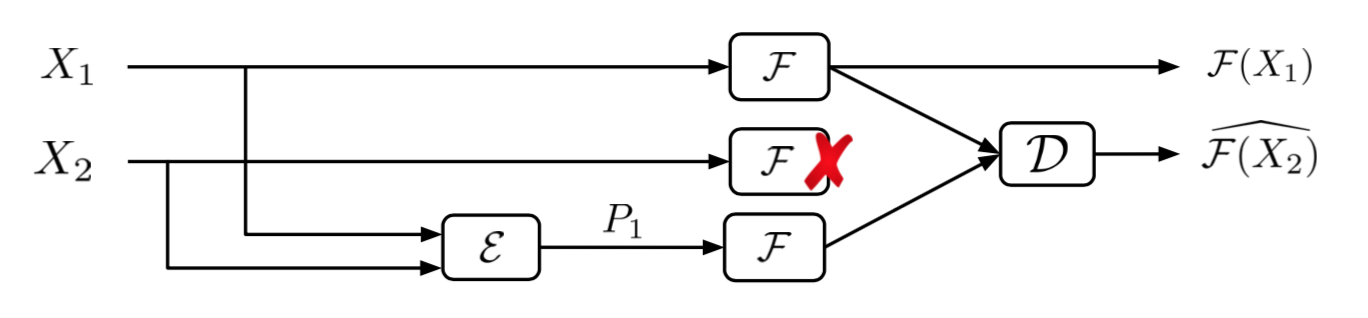
\includegraphics[width=0.8\textwidth]{./pf.png}
              \caption{Coded Computation}
            \end{figure}  
            
        Suppose there are $k$ data inputs $X_1, X_2, \cdots, X_k$, and suppose the goal is to apply a given function $\mathcal{F}$ to these $k$ data inputs, that is, to compute $\mathcal{F}(X_1),\mathcal{F}(X_2), \cdots, \mathcal{F}(X_k)$. The computations $\mathcal{F}(X_i),$ for different $i \in \{1,2,\cdots, k\}$ are performed on separate, unreliable devices, and hence each individual computation can straggle or fail arbitrarily. We let $r$ represent a resilience parameter. The framework of coded computation involves two functions, an encoding function $\mathcal{E}$ and a decoding function $\mathcal{D}$. First, the encoding function $\mathcal{E}$ acts on the $k$ data inputs $X_1, X_2, \cdots, X_k$ to generate $r$ redundant inputs, called "parities", which we denote as $P_1,P_2,...,P_r$. The given function $\mathcal{F}$ is then applied on these $(k + r)$ inputs (data and parity) on separate, unreliable devices that can fail or straggle arbitrarily. If any $r$ or fewer outputs (out of the total $(k + r)$ outputs) are unavailable, the decoding function $\mathcal{D}$ is applied on all the available outputs to reconstruct the unavailable ones among $\mathcal{F}(X_1),\mathcal{F}(X_2), \cdots, \mathcal{F}(X_k)$. Figure 1 illustrates the coded-computation framework. Given $\mathcal{F}$, $k$, and $r$, the goal is to design the encoding function $\mathcal{E}$ and the decoding function $\mathcal{D}$ to enable reconstruction of unavailable outputs of $\mathcal{F}$.
        
        \section{Project Objective}
        There are mainly two objectives:
        \begin{itemize}
            \item Complete implementing the basic algorithm of coded computation using neural networks to design the encoding function $\mathcal{E}$ and the decoding function $\mathcal{D}$
            \item Apply the algorithm on simulated data and make evaluations 
        \end{itemize}

        \section{Dataset}
        Gradient is an useful and important information in most machine learning algorithms. So to generate data for experiments, we choose the output of $\mathcal{F}$ to be gradients of different objective functions such as logistic function or probit function. We also mannually set the number of stragglers.
        
        \section{Experiment \& Result}
        For both $\mathcal{E}$ and $\mathcal{D}$, we use fully-connected neural networks with the same structure(same number of hidden layers and same number of nodes in each hidden layer) to construct the functions. The activation function for each hidden node is relu.
The output of $\mathcal{E}$ can be treated as a summary of all the data points of the current batch. The output of $\mathcal{D}$ is the approximation of the missing value.

        We simulated 10000 data points in total. Each data point is a $5 \times 1$ vector. We allocated 6 workers with $k = 5$ and $r = 1$. We also generated mask bits to mannually erase the straggler worker (0 for stragglers, 1 for normal workers). For training and testing, we used 5000 points as training data and the other 5000 points as testing data.
        \begin{table}[H]
        \centering
\begin{tabular}{@{}cccc@{}}
\toprule
\#hidden nodes & MAE         & MSE          & N-RMSE       \\ \midrule
5x500          & 0.0288 & 0.0190  & 0.0109   \\
6x500          & 0.0266 & 0.0131  & 0.0061  \\
7x500          & 0.0260 & 0.0061 & 0.0081  \\
8x500          & 0.0125  & 0.0066  & 0.0091  \\
9x500          & 0.0137 & 0.0068  & 0.0071 \\
10x500         & 0.0115 & 0.0078  & 0.0072 \\ \bottomrule
\end{tabular}
\caption{Test Error}
\label{tab:test-error}
\end{table}

Table \ref{tab:test-error} shows the testing error of the algorithm, including mean absolute error, mean square error and normalized root mean square error. With increasing number of hidden nodes, the error decreases. And the performance is obviously good.

        
        \section{Project Schedule}
            \begin{tabular}{cc}
                \hline
                Week & Assignment \\ \hline
                1& Set up experiment enviroment \\
                2& Build frame of algorithm \\
                3& Generate experiment data \\
                4& Debug \\
                5& Make evaluations \\
                \hline
            \end{tabular}

        \section{Inference}
        Kosaian, J., Rashmi, K.V. and Venkataraman, S., 2018. Learning a code: Machine learning for approximate non-linear coded computation. arXiv preprint arXiv:1806.01259.
            
        
            


\end{document}